\chapter{Methodology - Results / Is the Full Model Gradient a good Baseline?}
results comparing paraphrased setting and model generated setting

\fxnote{also include heatmap of similar gradients in results sections}
\fxnote{briefly explain all necessary notation and settings again}

\section{Performance of Gradient-Similarity as an Explanation Method}
\begin{table}[htb]
    \centering
    \begin{tabular}{|l|c|c|}
        \hline
        \textbf{Model} & \textbf{Paraphrased} & \textbf{Model-generated} \\
        \hline
        AMD-OLMo-1B-SFT & 0.993 & 0.218 \\
        \hline
    \end{tabular}
    \caption{Accuracy for the two settings: paraphrased and model-generated}
    \label{tab:model_accuracy}
\end{table}

\section{Single Layer Performance}

\begin{table}[htb]
    \centering
    \begin{tabular}{|c|c|c|c|}
        \hline
        & \textbf{Layer Component} & \textbf{Paraphrased} & \textbf{Model-generated} \\
        \hline
        \multirow{1}{5em}{Embedding}
        & Embedding & 0.993 & 0.231 \\
        \hline
        \multirow{4}{5em}{Attention}
        & Query-Projection & 0.979 & 0.253 \\
        & Key-Projection & 0.916 & 0.211 \\
        & Value-Projection & 0.982 & 0.188 \\
        & Output-Projection & 0.994 & 0.205 \\
        \hline
        \multirow{3}{5em}{MLP}
        & Gate-Projection & 0.994 & 0.265 \\
        & Up-Projection & 0.993 & 0.26 \\
        & Down-Projection & 0.995 & 0.221 \\
        \hline
    \end{tabular}
    \caption{Averaged (median) layer component accuracy \fxnote{also include mean}}
    \label{tab:average_accuracy_layer_component}
\end{table}

\fxnote{how "well" does each layer find the most relevant sample to paraphrased samples}
\fxnote{maybe create plot with averages per layer type (k proj, q proj, etc.)}

\section{Comparison of Layer-Gradients and Full-Model-Gradient}
\fxnote{Which layers are most similar to the full-gradient, e.g. MLP, ATTN, Embeddings?}

\begin{table}[htb]
    \centering
    \begin{tabular}{|c|c|c|c|}
        \hline
        & \textbf{Layer Component} & \textbf{Paraphrased} & \textbf{Model-generated} \\
        \hline
        \multirow{1}{5em}{Embedding}
        & Embedding & 0.981 & 0.275 \\
        \hline
        \multirow{4}{5em}{Attention}
        & Query-Projection & 0.972 & 0.275 \\
        & Key-Projection & 0.9 & 0.201 \\
        & Value-Projection & 0.978 & 0.62 \\
        & Output-Projection & 0.988 & 0.63 \\
        \hline
        \multirow{3}{5em}{MLP}
        & Gate-Projection & 0.986 & 0.553 \\
        & Up-Projection & 0.988 & 0.571 \\
        & Down-Projection & 0.989 & 0.63 \\
        \hline
    \end{tabular}
    \caption{Average (median) cosine similarity between the scores of single layer components and the full gradient}
    \label{tab:average_cosine_similarity_full_gradient_comparison}
\end{table}

\section{Greedy-Forward-Layer-Selection vs. Random Projections}

\subsection{Selection by Accuracy}

\begin{figure}[ht]
    \centering
    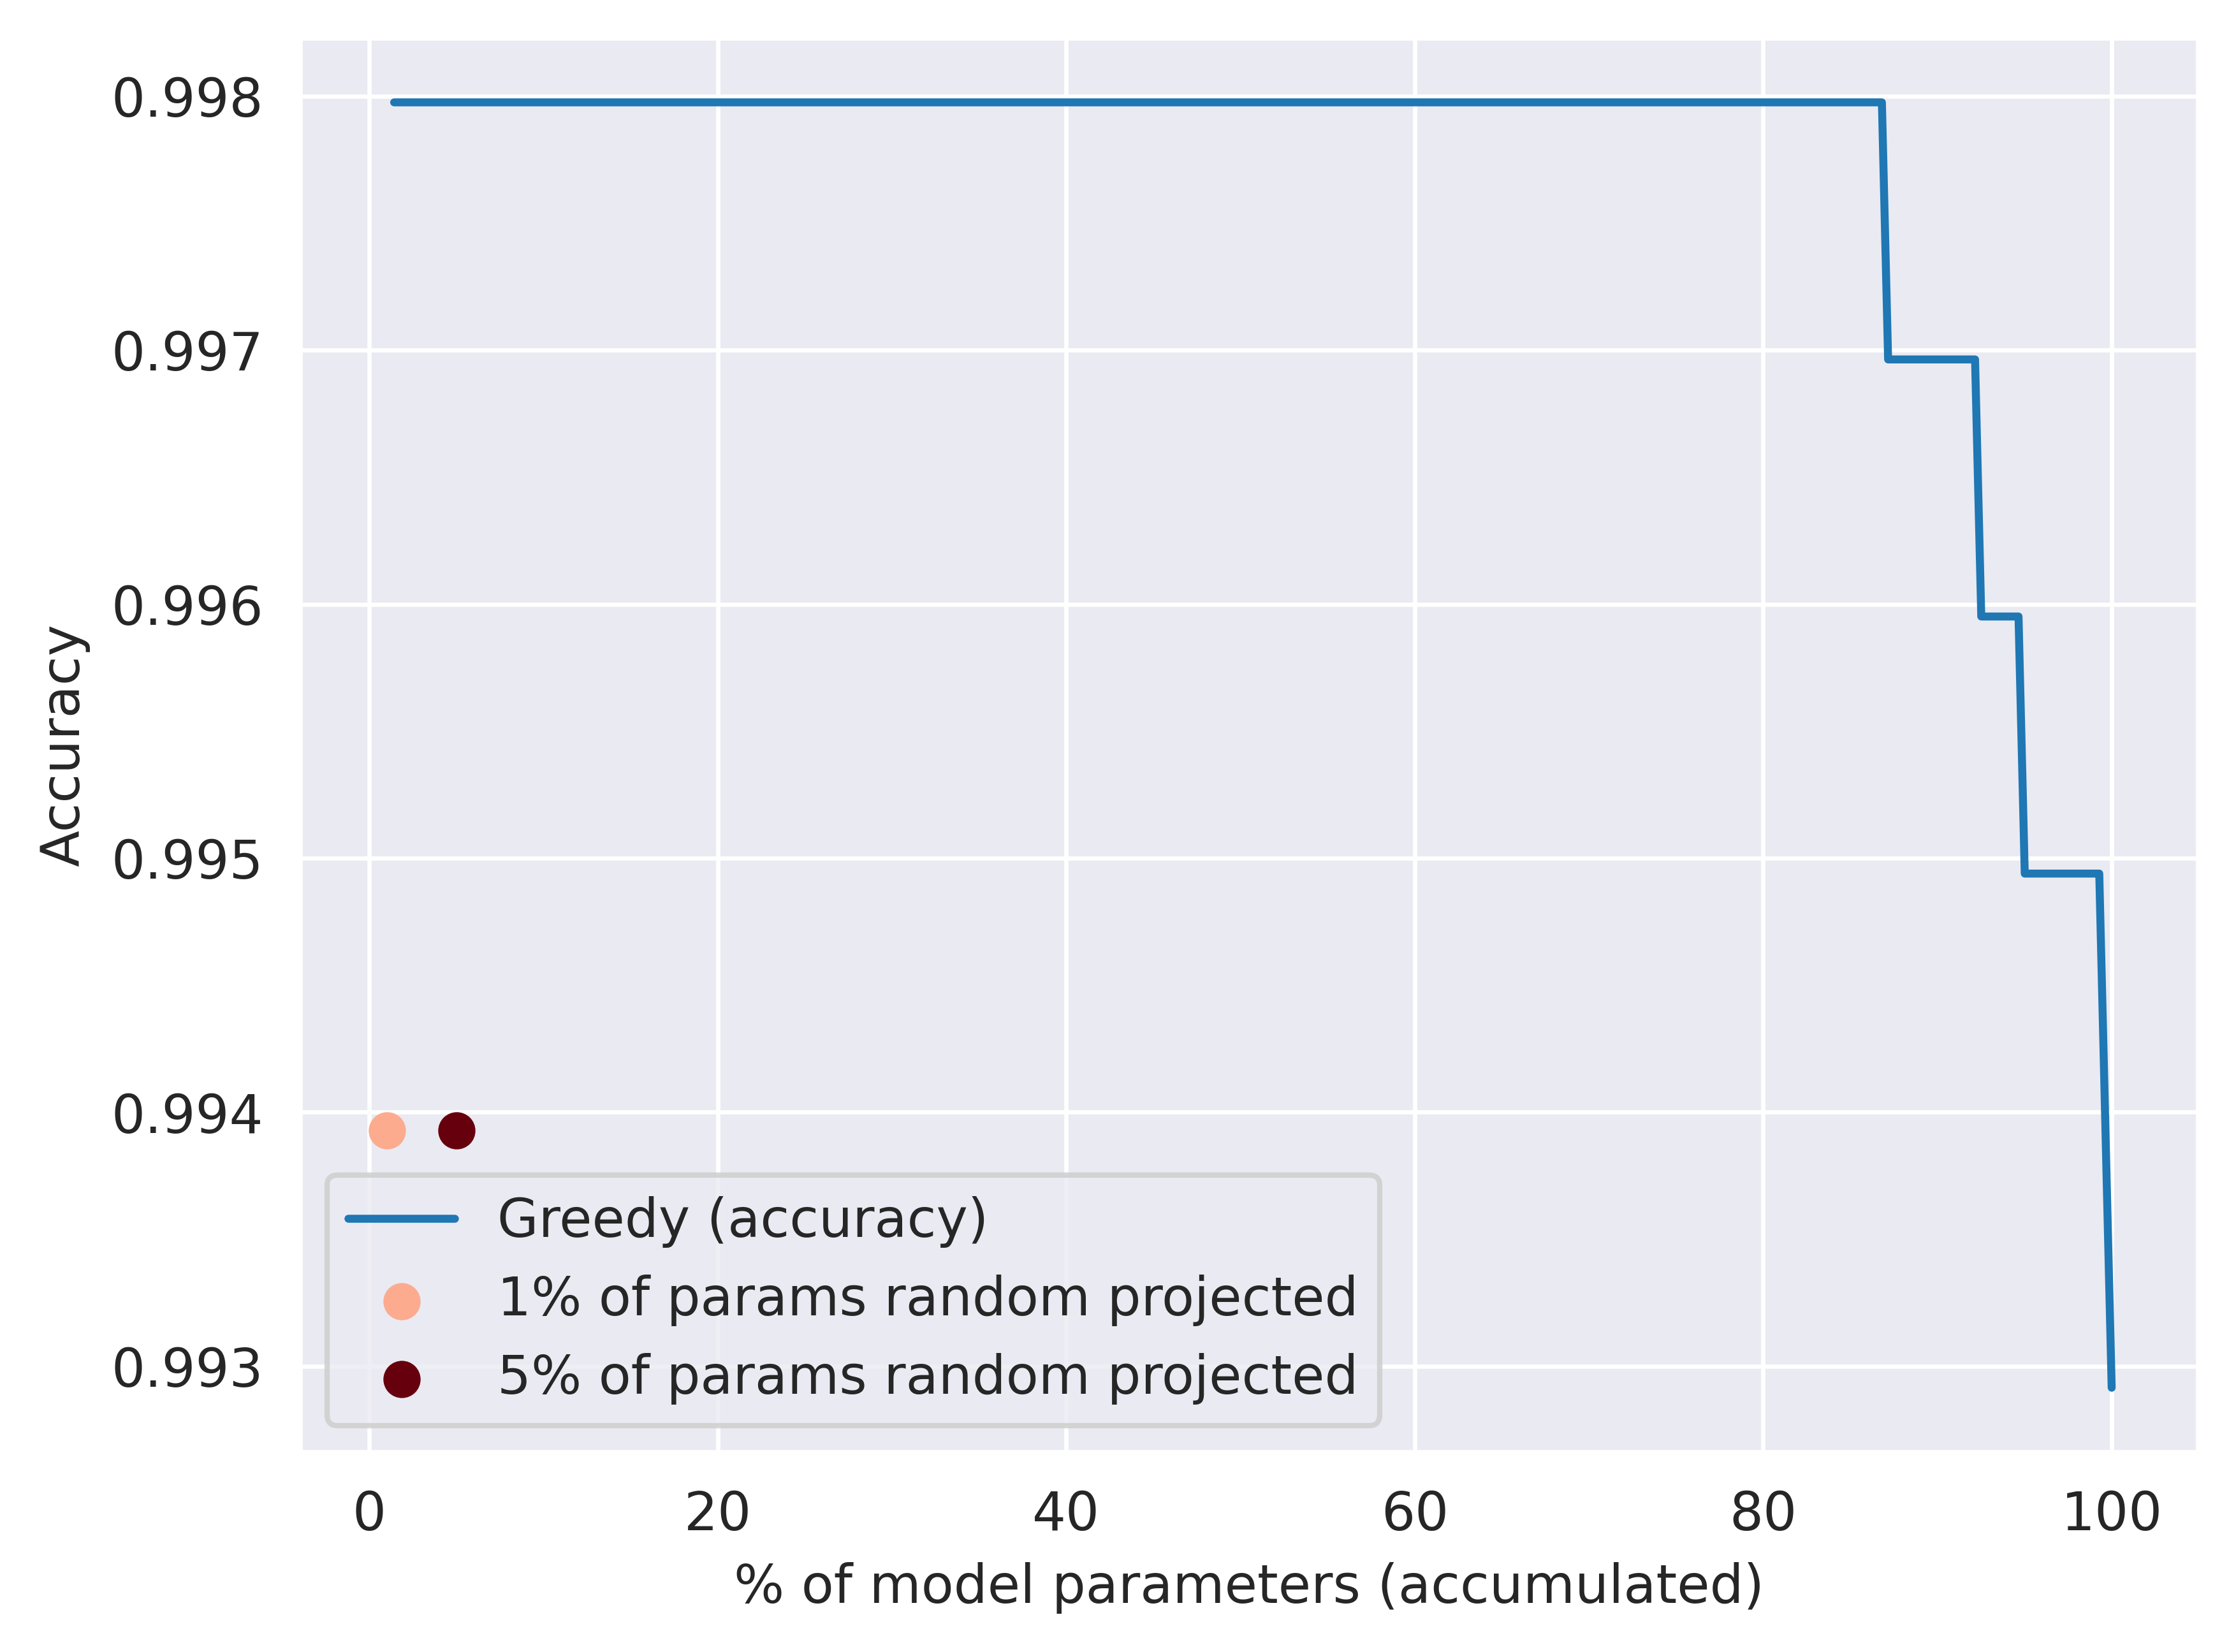
\includegraphics[width=1\textwidth]{figures/results/paraphrased/greedy_layer_selection_accuracy.png}
    \caption{Greedy Layer Selection and random projection by Accuracy (paraphrased)}
    \label{fig:greedy_layer_selection_accuracy_paraphrased}
\end{figure}

\begin{figure}[ht]
    \centering
    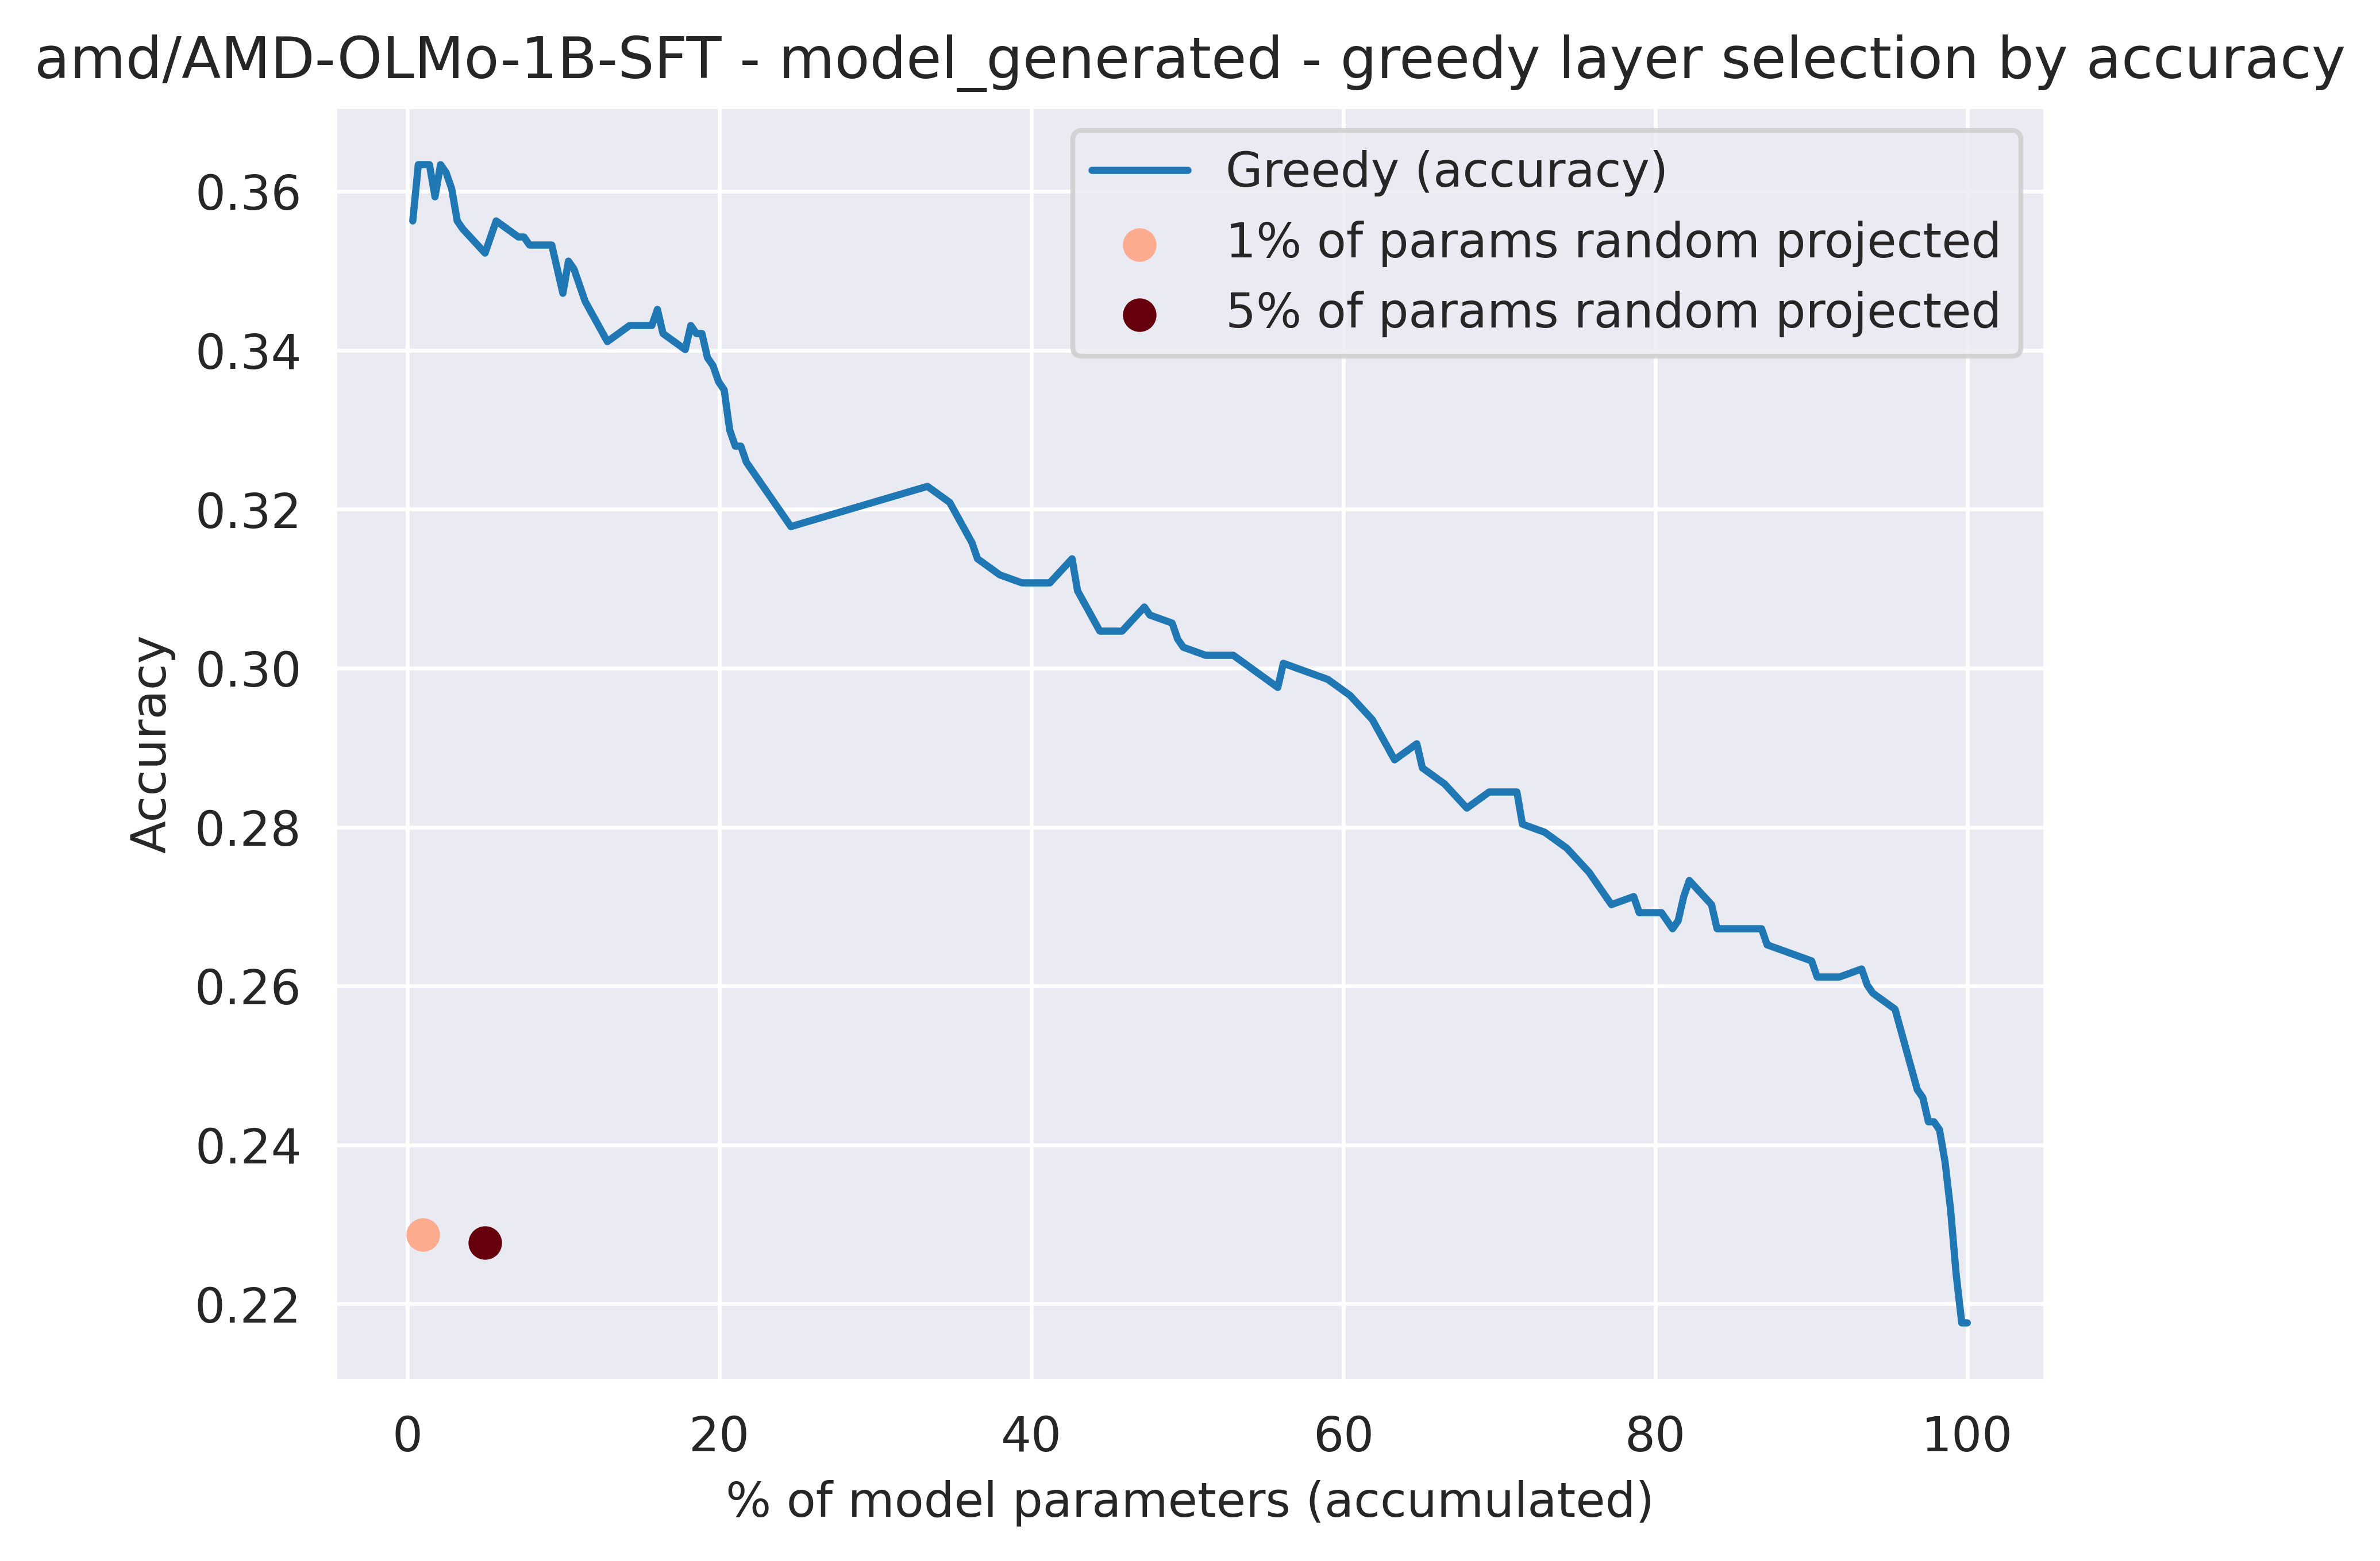
\includegraphics[width=1\textwidth]{figures/results/model-generated/greedy_layer_selection_accuracy.png}
    \caption{Greedy Layer Selection and random projection by Accuracy (model-generated)}
    \label{fig:greedy_layer_selection_accuracy_model_generated}
\end{figure}

\subsection{Selection by Similarity to Full-Model-Gradient}

\begin{figure}[ht]
    \centering
    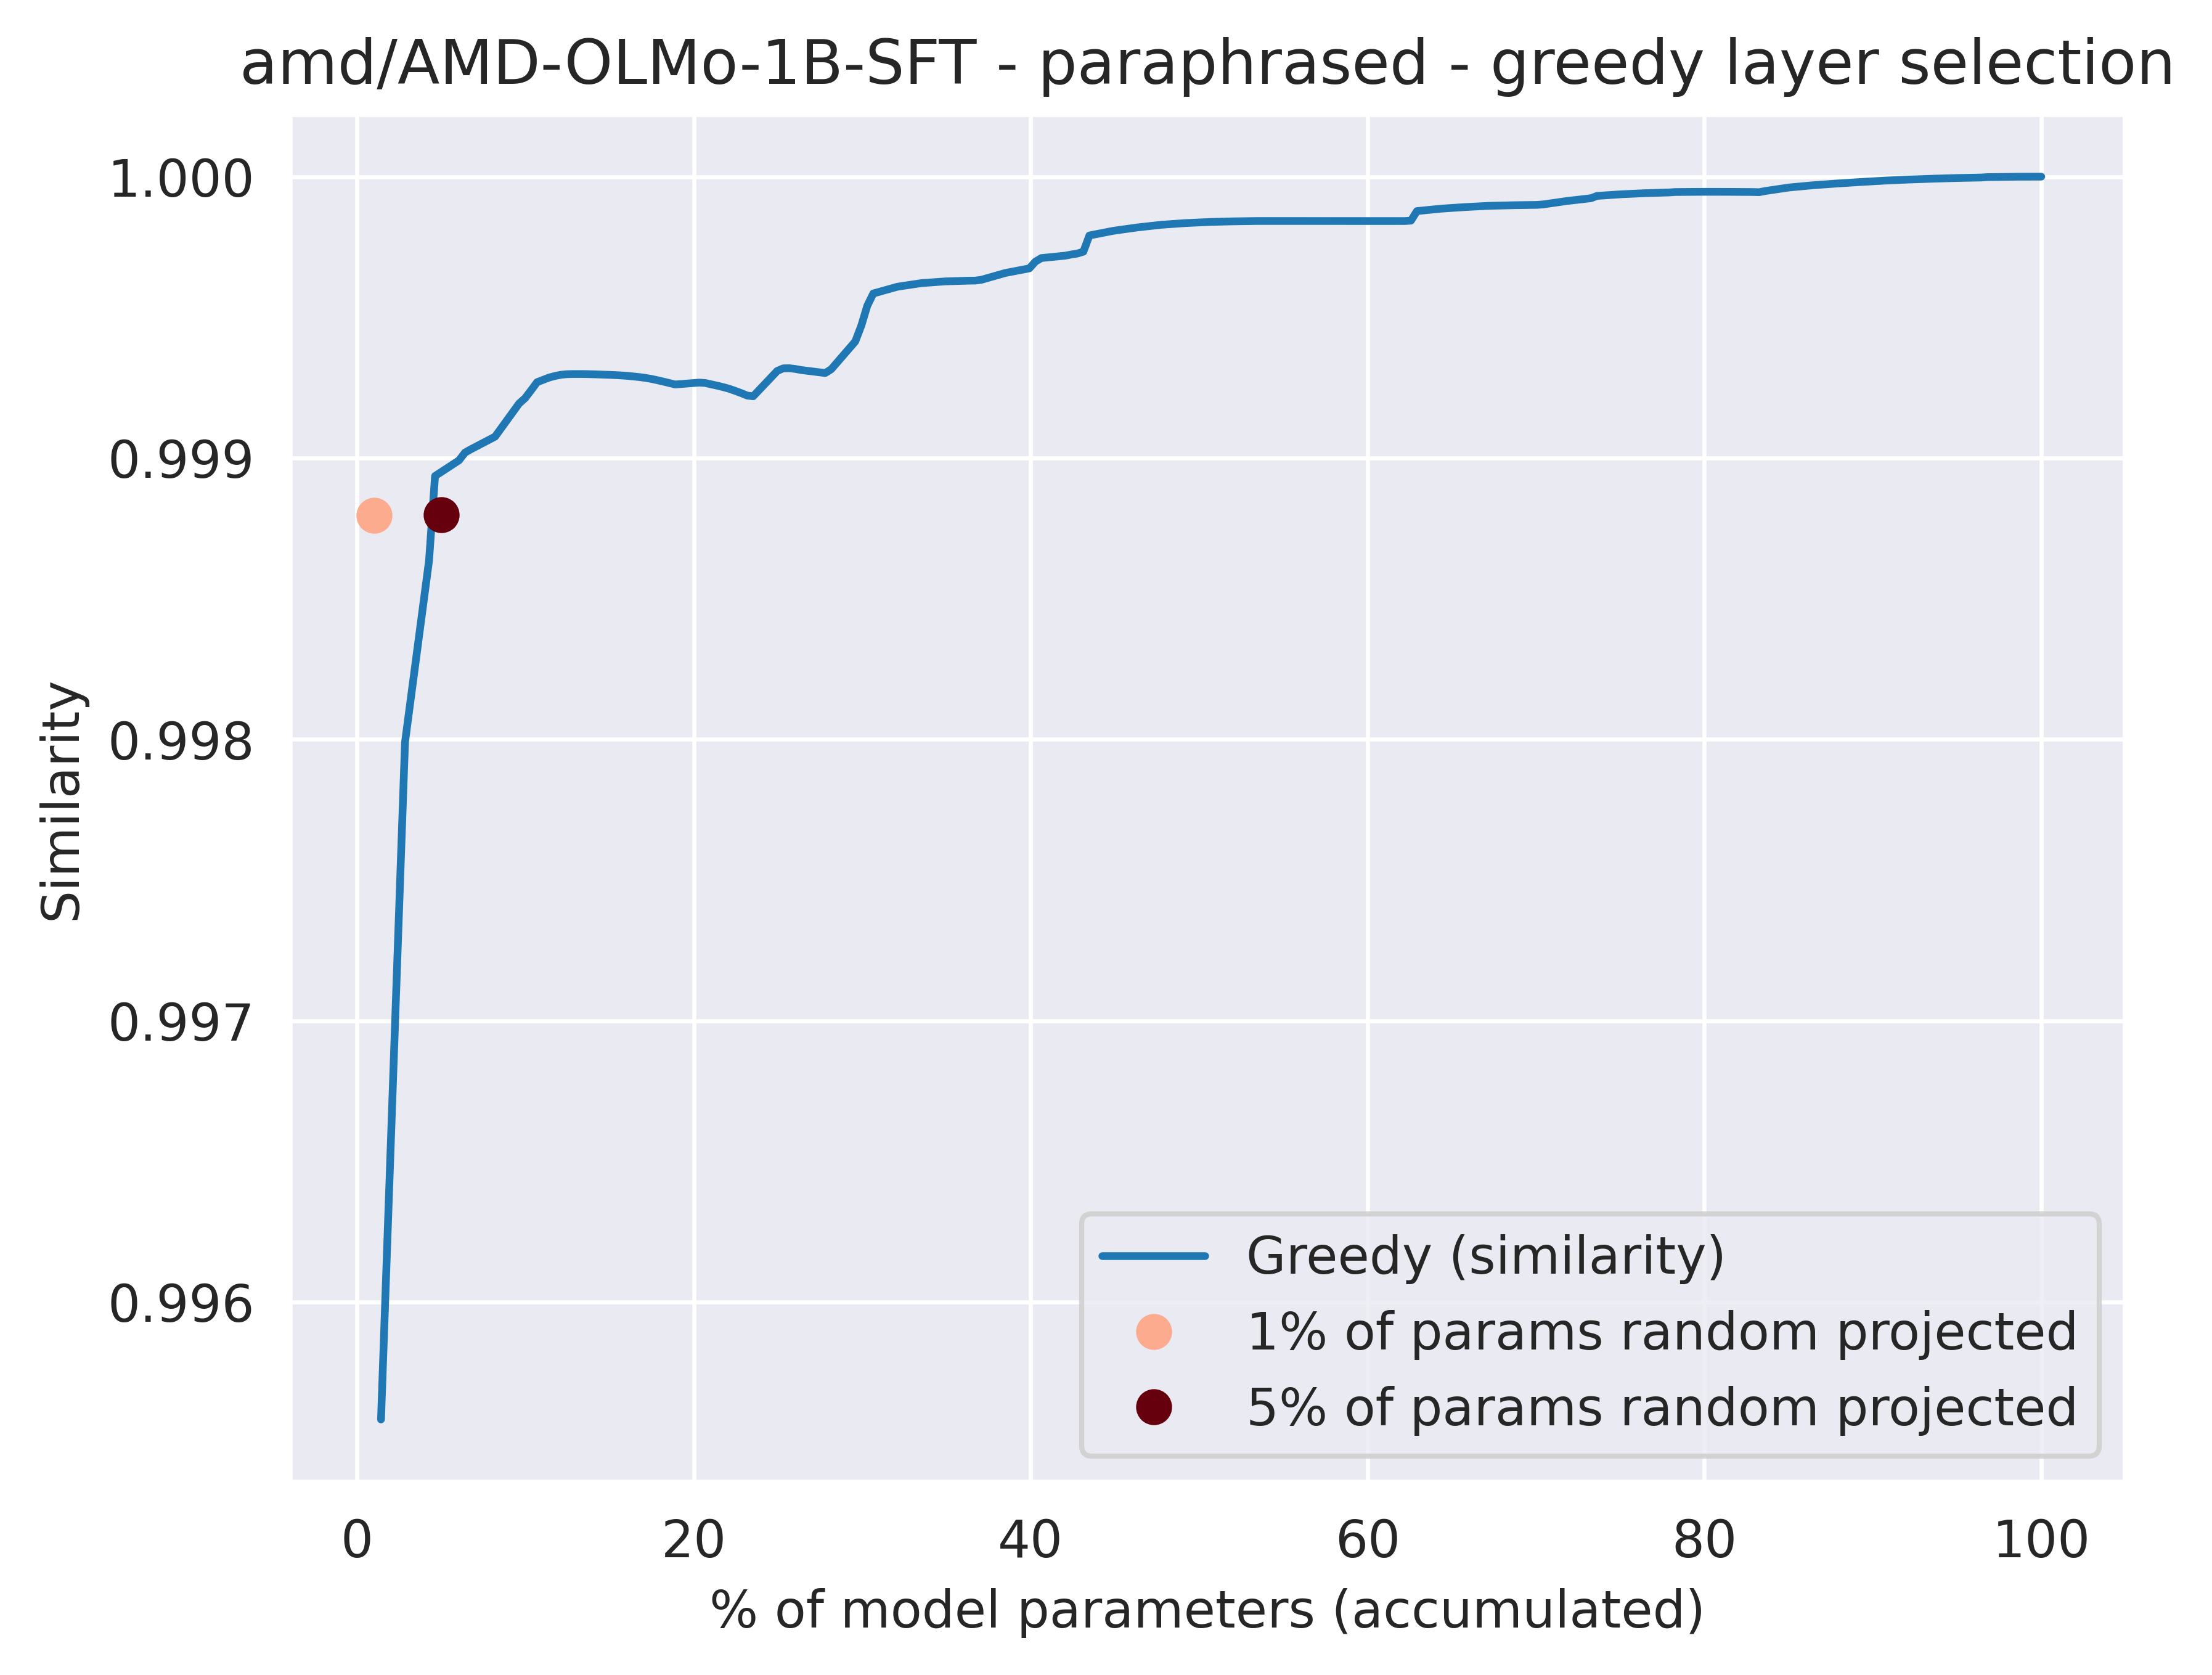
\includegraphics[width=1\textwidth]{figures/results/paraphrased/greedy_layer_selection.png}
    \caption{Greedy Layer Selection and random projection by Similarity to Full-Model-Gradient (paraphrased) }
    \label{fig:greedy_layer_selection_paraphrased}
\end{figure}

\begin{figure}[ht]
    \centering
    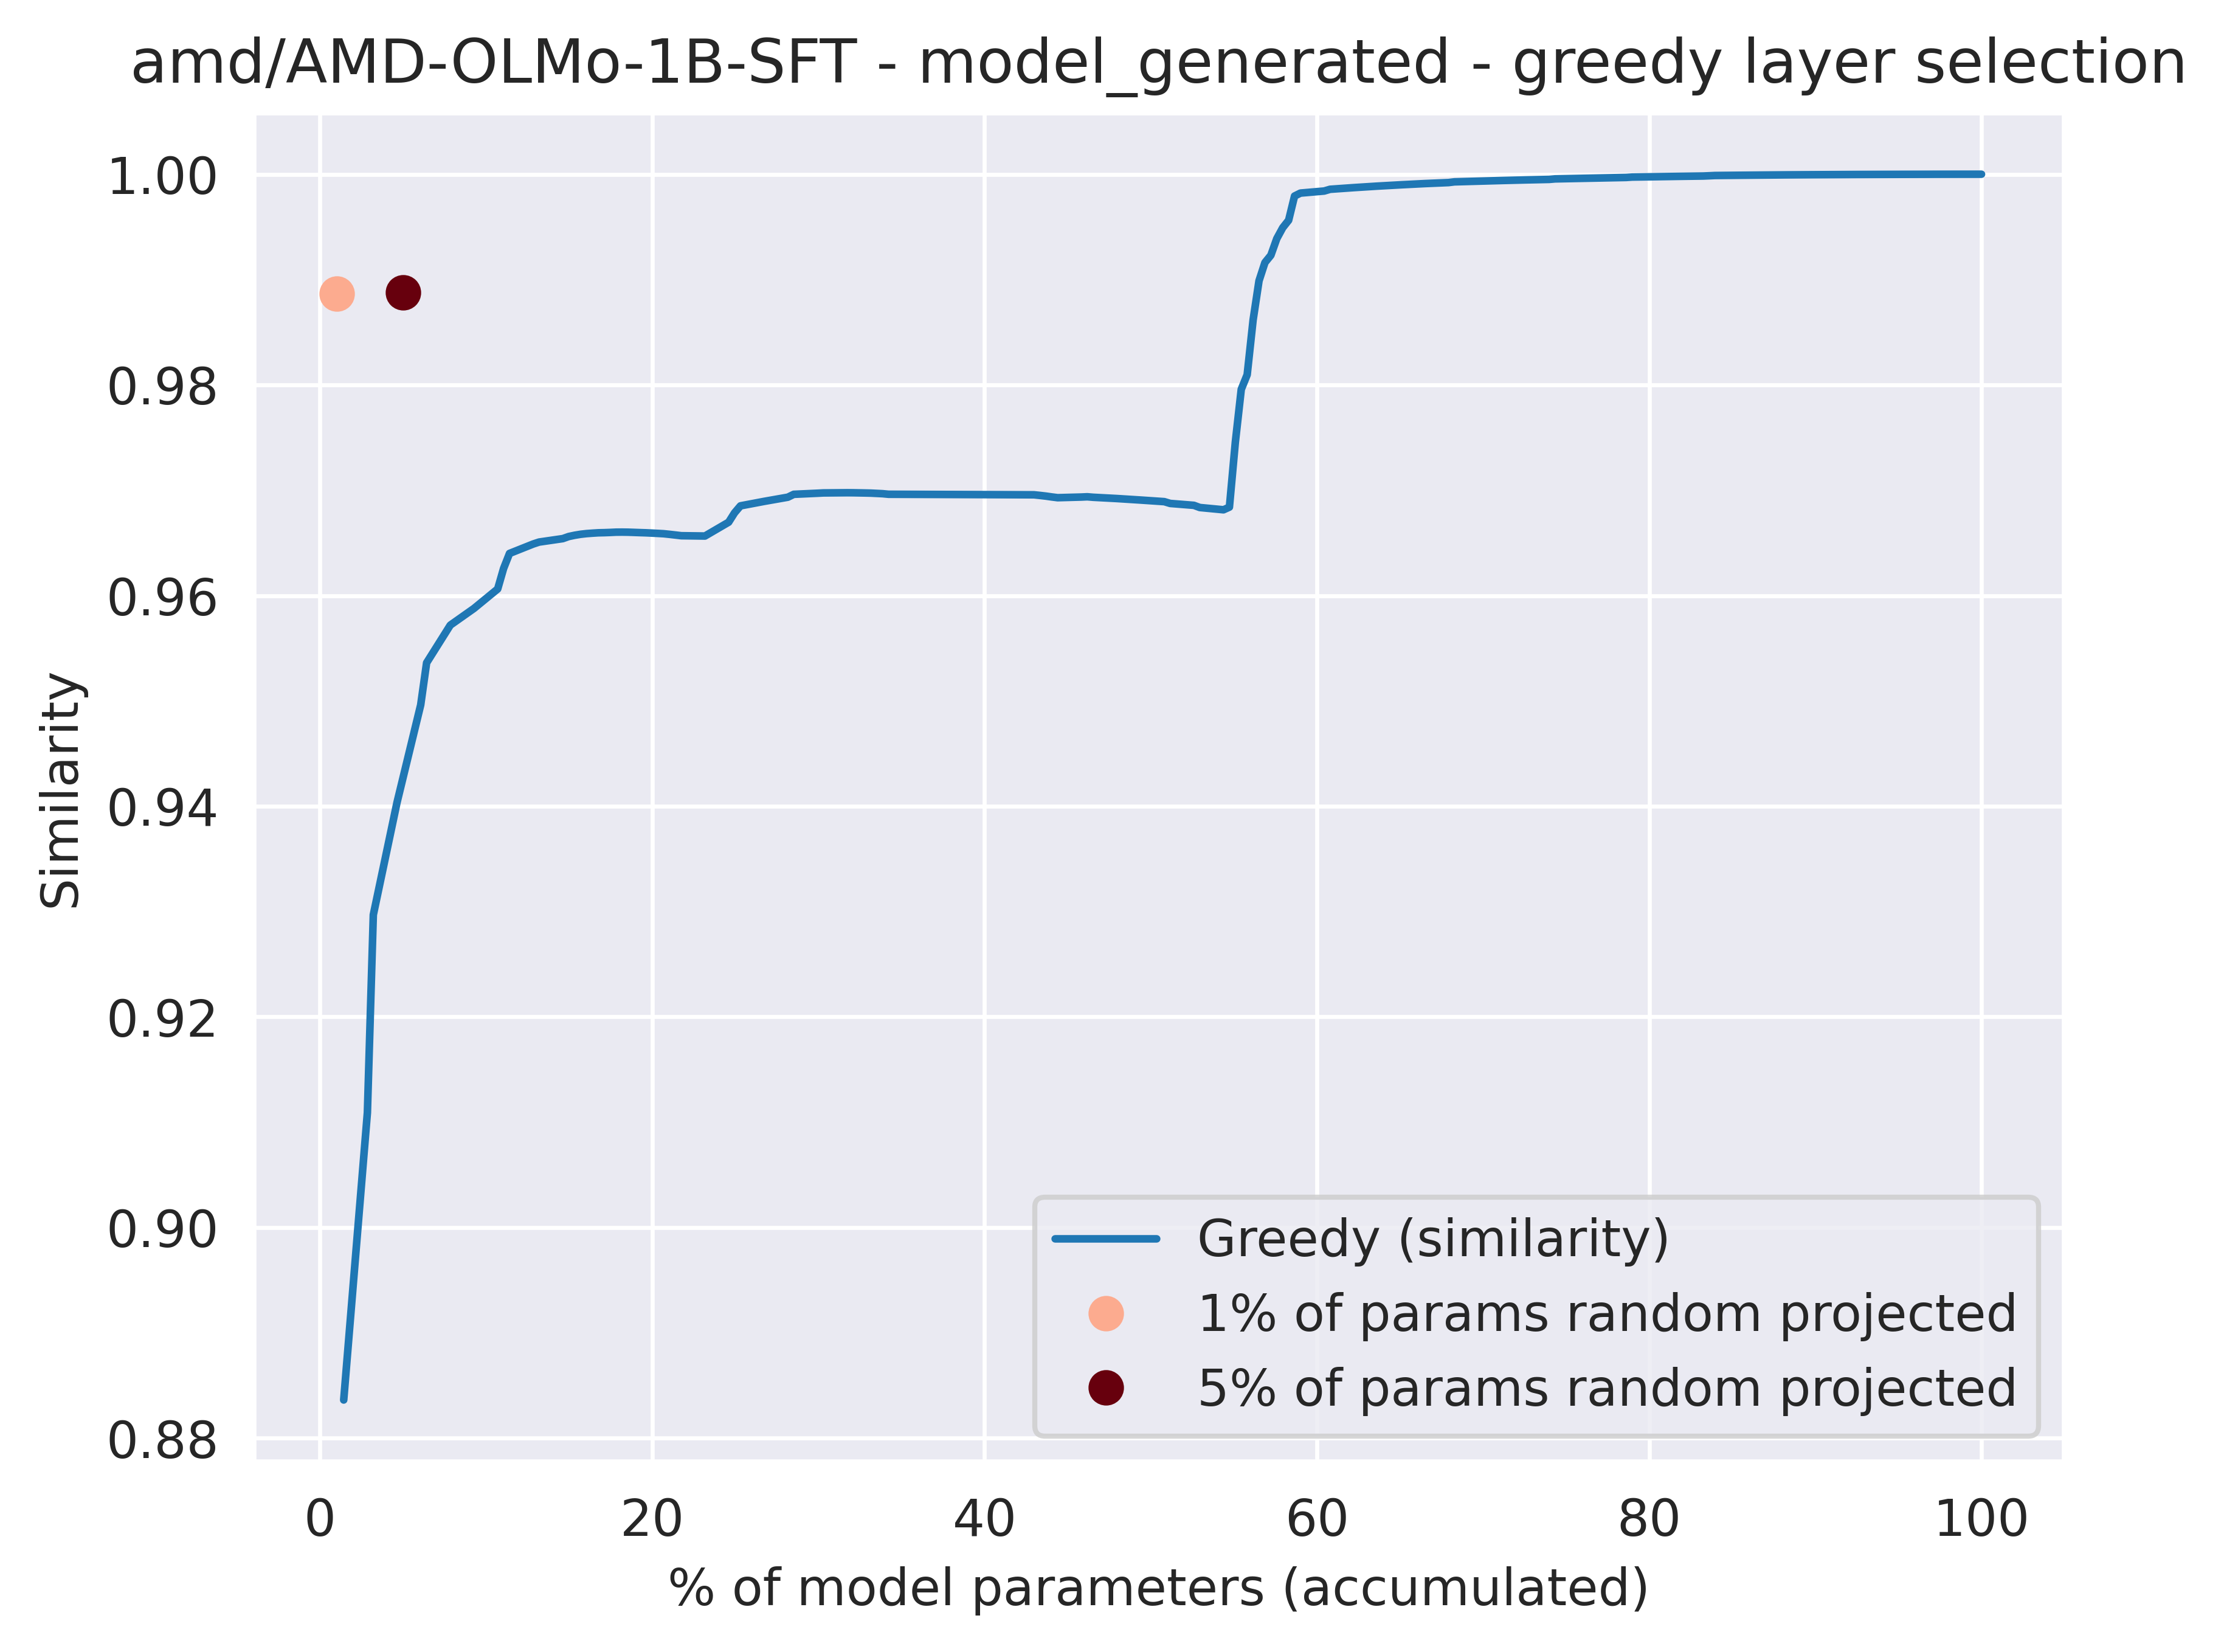
\includegraphics[width=1\textwidth]{figures/results/model-generated/greedy_layer_selection.png}
    \caption{Greedy Layer Selection compared to random projection by Similarity to Full-Model-Gradient (model-generated)}
    \label{fig:greedy_layer_selection_model_generated}
\end{figure}


\section{Execution Time}
The execution time is measured after the model and the tokenizer is loaded. Hence, it contains the time to load the dataset from the disk and perform all computations. Each \emph{Slurm} job logs its execution time separately and saves it on disk for later inspections. To make the results comparable, the individual times from the jobs are summed. Table~\ref{tab:execution_times} shows the execution times on the hardware described above described in Section~\ref{sec:hardware}. In this context, \emph{dot-products} refers to the computation of the intermediate dot-products mentioned in Subsection~\ref{subsec:intermediate_results} and \emph{gradient similarity} refers to the calculation of cosine similarities for the gradients. 
\begin{table}[htb]
    \centering
    \begin{tabular}{|l l|c|c|}
        \hline
        \textbf{Computation Type} & & \textbf{Paraphrased (h)} & \textbf{Model-generated (h)} \\
        \hline
        Dot-products & & 3.54 & 3.35 \\
        \hline
        \multirow{2}{*}{Gradient similarity} 
            & without RP & 4.05 & 5.39 \\
            & with RP & 927.48 & 925.63 \\
        \hline
    \end{tabular}
    \caption{Execution times (in hours) for dot-products and gradient similarity (with and without \acrfull{rp}) under paraphrased and model-generated settings.}
    \label{tab:execution_times}
\end{table}
